\chapter{Background}
Computer vision evolved from many complex theories, algorithms and models. This paper mainly talks 
about the video surveillance. This section helps to understand the required technical details confined to this area. 
\section{Optical Flow}
Optical flow can possibly be one of the most important concepts of computer vision. Optical flow is used 
to find the pattern in the movement of the objects from one frame to another. This is widely used in the 
fields like robotics, image processing, motion detection, object segmentation etc. Videos are the series of 
images. These images can be independent from one another. But, in the real time, a video captures 
consecutive change in the pixels in certain duration of time. There are many algorithms which discuss 
the relation between these pixels in two different frames. ~\cite{galvin1998recovering} discuss various 
types of optical flow algorithms and evaluates them. This paper concludes that Lucas Kanade Algorithm 
is best among the other 8 optical flow algorithms.

Optical flow diagrams are usually denoted by the vectors pointing the change from frame F1 to frame F2. But in real time, it is easy to concentrate on only those points which provide more insights. For example movement of the hand from F1 to F2 changes hundreds of pixels and can be redundant. Rather it is simple and more appropriate to see the flow of only those pixels at the corner of the hand. Thus, Corner detection algorithms are used to reduce the complexity and improve the performance of the algorithms.
\subsection{Corner Detection}
This paper trails 2 types of corner detection techniques to check the best possibility for the model.
\begin{itemize}
	\item Shi-Tomasi Corner detection.
	\item FAST Corner detection.
\end{itemize}
Shi Tomasi Corner detection algorithm is similar to Harris Corner Detector. it is widely used in detecting the interest points and feature descriptors. Interest points can be corners edges and blobs and are invariant to rotation, translation, intensity and scale changes. Only difference in harris corner detection and Shi Tomasi corner detection is the computed R value (used to detect the corner). 
FAST (Features from Accelerated Segment Test) on the other hand uses a different technique to predict not only the corners but also the edges based on the colour intensity and the threshold. 
\subsection{Lucas Kanade Algorithm}
In the conclusion of ~\cite{galvin1998recovering}, we can see that Lucas Kanade Algorithm is the one of the best algorithm to detect the optical flow. The assumption of Lucas Kanade algorithm is the flow of the local neighbourhood of the pixel is constant. It combines all the information from the surrounding pixels and often solves the inherent ambiguity of the optical flow equation. It is also considered to be less sensitive to the noise.
\section{Density based clustering}
Clustering in general is combining a group of similar objects based on their similarities like shape, angle, magnitude and position. In order to reduce the memory consumption of the CPU/GPU it is important to consider those points which are critical to the analysis. Thus, clustering the points and vectors based on the position and direction helps to combine the similar points and vectors to predict the movement of the crowd. In this paper we have considered using 2 types of density based clustering.
\begin{itemize}
	\item DBSCAN.
	\item OPTICS.
\end{itemize}
\section{Convolutional Neural networks}
Convolutional neural networks are the advanced concept of neural networks which gives computers the ability to understand the images and videos. CNNs currently are being used in a wide range of application like Robotics, Face detection, Crowd detection, Weather study, Advertising, Environmental studies etc. Every neurone in the CNN has the learnable weights. They are initialised with random weights and can be trained to develop a model. CNN are comprised of below 3 topics.
\begin{itemize}
	\item Convolution Networks (ConvNets).
	\item Pooling.
	\item Fully Connected Layers.
\end{itemize}
\subsection{Convolution Networks (ConvNets)}
Convolution Networks also called as ConvNets is the process of changing the pixels of the image using filters. The image is a matrix of pixels and a filter/kernel is used to alter the pixel value with matrix multiplication. This filter is applied on the whole image by striding through the image. There are different filters for different types of results. 
\subsection{Pooling}
Pooling is the process of reducing the size of the image with the help of a filter. The pooling is usually of 2 types, Average pooling and Max pooling. Image is reduced to a desired size by the filter by taking the average of the pixels or Max pixel depending on the pooling technique.
\subsection{Fully Connected Layers}
Fully connected layers are the neural networks which has the 1D array of the ConvNets as the inputs and a series of different hidden layers which are fully connected. The output of these networks are the classification nodes which can either be integers or One Hot encoded values predicting the classification. The prediction of the classification is usually done by SoftMax (Picks the highest probability node).
\subsection{Notable CNN Architectures}
There are few CNN architectures which are available as the modules. These modules are pre-trained and can be directly implements provided the inputs and outputs are exactly same as expected by the module. PyTorch library can be explored to find the list and implementation of these networks. This project implements below 3 CNN architectures.
\begin{itemize}
	\item AlexNet
	\item VGG
	\item ResNet
\end{itemize}
\subsection{AlexNet}
AlexNet CNN architecture was first proposed in \cite{krizhevsky2012imagenet} by Alex Krizhevsky in the year 2012. The architecture diagram \ref{fig:AlexNet} of the Alexnet gives the insight of the depth and the processing of the CNN. AlexNet contained 8 layers, among them 5 were convolution layers followed by Max pooling and the last 3 layers were the fully connected layers. Alex net was considered to be one of the most famous architectures at that time. It uses non saturating ReLu function which can be changed to tanh and sigmoid functions to improve the performance.
\begin{figure}[tb]
	\center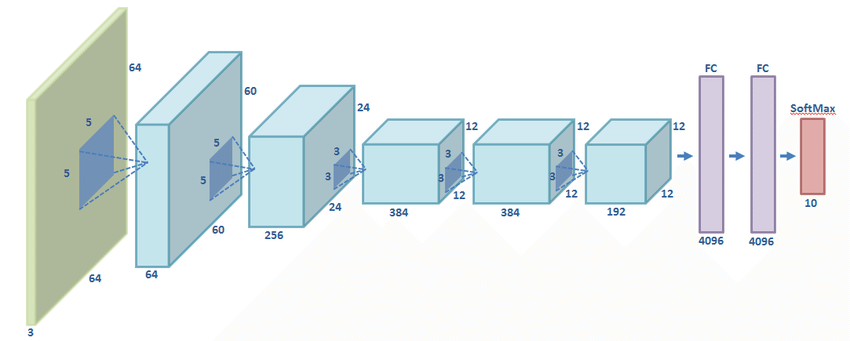
\includegraphics[width=0.6\textwidth]{AlexNet.png}
	\caption{AlexNet Architecture \cite{article}}
	\label{fig:AlexNet}
\end{figure}

\subsection{VGG}
VGG architecture was first proposed in \cite{simonyan2014very} by Karen Simonyan in the year 2015. As per this paper there are 4 variations (vgg11, vgg13, vgg16 \& vgg19) in the architecture depending on the depth of the networks. Vgg architecture takes an input of 224*224*3 image and pass it through different convolution layers followed by Max pooling. This paper implements vgg11 architecture and this architecture is different from the AlexNet as described in \ref{fig:vgg11}.

AlexNet architecture has max pool layer after every convolutional layer, but in VGG architecture there is a difference in the placement of the Max pool layer some times after a series of 2 or 3 convolutional layers. This helps to retain the feature information before reducing the size through max pooling. towards the end of the architecture there are 3 layers of fully connected networks to classify different outputs.
\begin{figure}[h!]
	\center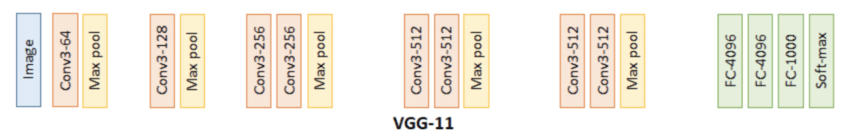
\includegraphics[width=0.6\textwidth]{vgg11.png}
	\caption{VGG 11 Architecture \cite{vgg11}}
	\label{fig:vgg11}
\end{figure}
  
\subsection{ResNet}
ResNet is residual neural network which is build on constructs known from pyramidal cells in the cerebral cortex. In order to achieve this property it uses skip connections over some layers. The model is implemented with double or triple skips using ReLu and batch normalisation. ResNets are built on the idea that the added more layers to the CNN architectures will not reduce the error rather just increase the computation cost. This is the reason, this model proposes to use the skip connects to reach to the lower layers faster when required by preserving the feature characteristics. The skip connections are described in the figure \ref{fig:resnetskip}
\begin{figure}[h!]
	\center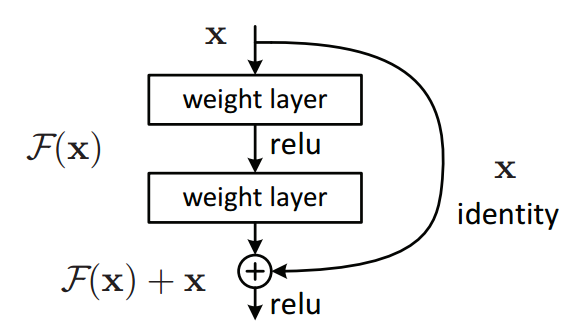
\includegraphics[width=0.6\textwidth]{resnetskip.png}
	\caption{ResNet Skip connections \cite{resNet}}
	\label{fig:resnetskip}
\end{figure}

\section{Machine Learning Models}
There are 3 types of machine learning algorithms: Supervised learning, Unsupervised learning and reinforcement learning. Supervised learning works on the concept of learning from the previous experiences. In this case, the models are trained with the help of labelled data. The model trains from the inputs and is implemented on the fresh data to check the model accuracy. Unsupervised learning is the concept of leaning based on the input information with out any previous experience. In this case of learning the models are fed with large amounts of data and the model plots the data to find the similarities in the placement, pattern recognition and prediction. The third type of machine learning approach is the reinforcement learning where the machine is exposed to an environment where it trains itself continually using trial and error.

This project deals with the classification models and implements the classification ML models under supervised learning. The data is trained using the following models:
\begin{itemize}
	\item Logistic Regression
	\item Support Vector Machines
	\item K nearest neighbours
	\item Gaussian Naive Bayes
	\item Perceptron
	\item Stochastic Gradient Descent
	\item Decision Tree
	\item Random Forest
\end{itemize}

\subsection{Logistic Regression}
Logistic Regression is used to estimate the discrete values based on the inputs provided. Logistic regression can be implemented in multiple ways depending on the requirement. in Simple logistic regression, the classification is binary. where as in the multi-nominal logistic regression the output can be multiple classes. The idea of the logistic regression is developed from the linear regression where the model defines a linear function to predict the value. But in case of classification all the values are either 0 or 1. In this case the best fit cannot be a linear function, rather it uses the sigmoid function to predict the values as shown in \ref{fig:logisticregression}. The derivation of the Logistic regression likelihood function is as follows.
 \begin{equation}\label{eqn:linear}
    y = mx + c
 \end{equation}
 \begin{equation}\label{eqn:sigmoid}
    \sigma(y) = \frac {1}{1+ e^{-(mx + c)}}
 \end{equation}


\begin{figure}[h!]
	\center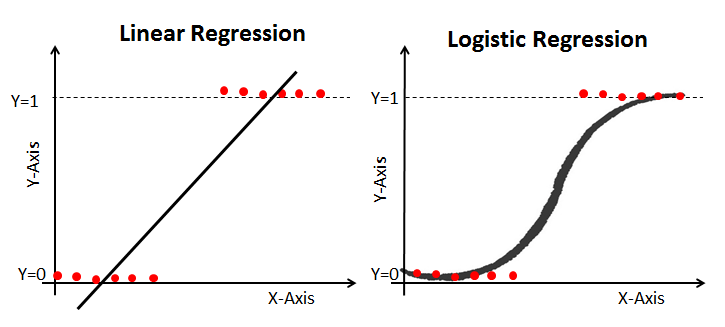
\includegraphics[width=0.6\textwidth]{logisticregression.png}
	\caption{Linear Regression Vs Logistic Regression \cite{logistic}}
	\label{fig:logisticregression}
\end{figure}
 
\subsection{Support Vector Machines}
Support vector machines is used to classify the data into groups and generally works on the supervised dataset. It plots every point of the data in the n  dimensional plot. Where n being number of features. As all the data is plotted in n dimensions, the algorithm works to split the data into the different classes based on the plot. The SVMs are considered to be one of the best classification algorithms.

\subsection{K nearest neighbours}
K nearest neighbours algorithm is one of the simple algorithm which takes the parameter k. The value k defines the clustering the data based on the distance function. There are many types of the distance functions namely: Manhattan, Euclidean, Minkowski and Hamming distance. Among these distance functions, hamming is used for the classification problems. KNN algorithm is considered to be computationally expensive, specially to work on a larger dataset. Basic idea is to calculate the distance matrix of all the points and classify them based on the number of classes with a threshold value.

\subsection{Gaussian Naive Bayes}
Gaussian Naive Bayes technique is based on the Bayes theorem which is built on the assumption that the predictors are completely independent. Naive Bayes theorem is simple to calculate and is known for its simplicity yet very efficient model. The theorem is based on calculating the posterior probability P(c|x) from P(c), P(x) and P(x|c) as mentioned in the equation \ref{eqn:bayes}
 \begin{equation}\label{eqn:bayes}
    P(c|x) = \frac {P(x|c) P(c)} {P(x)}
 \end{equation}

\subsection{Perceptron}
Perceptron algorithm is considered to be the best algorithm to be used on the linearly separable data. Perceptrons are the 3 layer neural networks where the inputs are the features and the middle layer takes the weighted sum of the inputs and applies a function and gives an output. This output is compared with the actual value and the loss is back propagated to change the weights. After multiple calculations, the algorithm returns the values with less error and thus nearly fit to the classification problem.

\subsection{Stochastic Gradient Descent}
Stochastic Gradient Descent works on the concept of Gradient Descent algorithm. This can be called as the modified Gradient Descent which tackles the problem of computation logic. In gradient descent, every instance is used to calculate the best fit of the model. This can be cost consuming in case of many samples. In order to reduce this computation problem, SGD uses the batch selection process where it uses one record from each batch for the computation of the best fit. SGD is a considered to be a good model on large number of data with redundant values.

\subsection{Decision Tree}
Decision tree model is one of the most frequently used classification model. It can be used both on the categorical and continuous target variables. This model works on the bases of splitting the data based on a category. The main components of decision tree are as follows

\begin{itemize}
	\item Root Node: It is the base node of the tree and generally represents the total population.
	\item Splitting: It is a process of dividing a node into two or more sub-nodes.
	\item Decision Node: The node which is split into sub nodes
	\item Leaf Node: The node which do not split into further nodes.
	\item Pruning: Reducing the sub nodes of the decision tree.
	\item Branch: It is the sub tree of the decision tree.
\end{itemize}

There are different types of splitting. But in general the splitting is done on the bases of 2 algorithms Gini and Information Gain. Gini is the probabilistic way of splitting the node into binary nodes by calculating the square of probability of success and failure of the sub nodes. It then uses the weighted Gini score on the each node to split the nodes. On the other hand the Information gain works on calculating the entropy on each class and further calculate the information gain on each class. Depending on the information gain, it splits the node into sub nodes.

\subsection{Random Forest}
Random forest is the collection of multiple decision trees algorithm. It classifies the class with most outputs from the different decision trees. The basic algorithm works by row sampling and feature sampling the dataset to multiple decision trees. This is bootstrap of the data to multiple decision trees and get the output from all the trees. Now the aggregation works on the outputs of different decision trees and picks the class with more predictions from the decision trees.

 
 


  

